\documentclass[11pt]{article}

\usepackage{a4wide}
\usepackage{amsmath,amssymb}
\usepackage[english]{babel}
\usepackage{enumitem}
\usepackage{float}
\usepackage{graphicx}
\usepackage[utf8]{inputenc}
\usepackage{listings}
\usepackage{multicol}
\usepackage{tikz}

%========== DEFINITIONS & MACROS ==========%

\definecolor{comment}{rgb}		{0.38, 0.62, 0.38}
\definecolor{keyword}{rgb}		{0.10, 0.10, 0.81}
\definecolor{identifier}{rgb}	{0.00, 0.00, 0.00}
\definecolor{string}{rgb}		{0.50, 0.50, 0.50}

\newcommand{\appref}[1]{see appendix \ref{#1} on page \pageref{#1}}
\newcommand{\txtref}[2][]{see {\it #1} \ref{#2} on page \pageref{#2}}
\newcommand{\code}[1]{{\tt #1}}
\newcommand{\file}[1]{{\tt #1}}
\newcommand{\imp}{\rightarrow}
\newcommand{\norm}[1]{\lVert#1\rVert}

\setdescription{leftmargin=\parindent, labelindent=\parindent}

\lstset
{
    language=C++,
	% general settings
	numbers=left,
	frame=single,
	basicstyle=\footnotesize\ttfamily,
	tabsize=2,
	breaklines=true,
	% syntax highlighting
	commentstyle=\color{comment},
	keywordstyle=\color{keyword},
	identifierstyle=\color{identifier},
	stringstyle=\color{string},
}


\title
{
    {\Large Individual Assignment 2} \\
    Introduction to Computer Graphics
}

\author
{
    Casper B. Hansen \\
    University of Copenhagen \\
    Department of Computer Science \\
    {\tt fvx507@alumni.ku.dk}
}

\date{last revision \today}

\begin{document}

\clearpage\maketitle\vspace{1in}
\begin{multicols}{2}
    \begin{abstract}
        We discuss the subject of geometric transformations in relation to
        computer graphics. In solving how we may perform such transformations,
        we look at how we can represent it in a convenient way and apply this
        to further develop how we can produce a uniform mathematical procedure
        by which we can arrive at the conclusion of how this translates into
        practice by concatenating such transformations. Finally we look at a
        possible implementation of geometric transformations in a 3D
        engine environment.
        
        The reader is not expected to have any prior knowledge of the material
        presented. For the code the reader is expected to have some basic
        understanding of linear algebra  and the C++ language.
    \end{abstract}
    \vfill\columnbreak\tableofcontents\vfill
\end{multicols}
\thispagestyle{empty}\newpage

\section{The Problem}
We seek a convenient mathematical expression that combines the properties of
an object, and a uniform way of the transformation thereof.

\subsection{Transformations}
In our endeavor to produce these formulae, we must first define the
transformations we require.
\begin{description}
    \item[Translate] displaces points by a vector.
    \item[Rotate] displaces points by rotating them around an axis by an
    angle.
    \item[Scale] displaces points by multiplying each component of the point
    by scale factors.
    \item[Shear] displaces points by stretching them along an axis.
\end{description}

\subsection{Euclidean Coordinates}
In solving this, we consider an obvious choice of representation; for a point
$p$ in 2-dimensional space, we represent this in Euclidean coordinate space as
$(p_x, p_y)^T$ --- note $p \in \mathbb{R}^2$.

\begin{multicols}{2}
    
    \subsubsection{Translation}
    Given a point $a$, the translation tranformation of point $a$ by point
    $t$, producing the point $b$ is given by
    \small
    \begin{align}
        \begin{bmatrix}
            b_x \\
            b_y
        \end{bmatrix}
        &=
        \begin{bmatrix}
            a_x \\
            a_y
        \end{bmatrix}
        +
        \underbrace{
        \begin{bmatrix}
            t_x \\
            t_y
        \end{bmatrix}}_{\text{\bf t}}
        =
        \begin{bmatrix}
            a_x + t_x \\
            a_y + t_y
        \end{bmatrix}
    \end{align}
    \normalsize
    Or, more compactly $b = a + \text{\bf t}(t_x, t_y)^T$.
    
    Notice that this transformation is additive, not multiplicative, as the
    other transformation operations, as follows.
    
    \subsubsection{Rotation}
    Given a point $a$, the rotation transformation of point $a$ around an axis
    by an angle $\theta$, producing the point $b$ is given by
    \small
    \begin{align}
        \begin{bmatrix}
            b_x \\
            b_y
        \end{bmatrix}
        &=
        \underbrace{
        \begin{bmatrix}
            \cos \theta     & \sin \theta \\
            -\sin \theta    & \cos \theta
        \end{bmatrix}}_{\text{\bf R}(\theta)}
        \begin{bmatrix}
            a_x \\
            b_y
        \end{bmatrix} \\ \nonumber
        &=
        \begin{bmatrix}
            a_x \cos \theta - a_y \sin \theta \\
            b_x \sin \theta - a_y \cos \theta
        \end{bmatrix}
    \end{align}
    \normalsize
    Or, more compactly $b = \text{\bf R}(\theta) a$.
    
    \vfill\columnbreak
    
    \subsubsection{Scaling}
    Given a point $a$, the scaling tranformation of point $a$ by scale factors
    $s$, producing the point $b$ is given by
    \small
    \begin{align}
        \begin{bmatrix}
            b_x \\
            b_y
        \end{bmatrix}
        &=
        \underbrace{
        \begin{bmatrix}
            s_x & 0 \\
            0   & s_y
        \end{bmatrix}}_{\text{\bf S}}
        \begin{bmatrix}
            a_x \\
            a_y
        \end{bmatrix}
        =
        \begin{bmatrix}
            s_x a_x \\
            s_y a_y
        \end{bmatrix}
    \end{align}
    \normalsize
    Or, more compactly $b = \text{\bf S}(s_x, s_y) a$.
    
    \subsubsection{Shearing}
    Given a point $a$, the shearing transformation of point $a$ by the shear
    factors $s$, strecthing the point along an axis, producing the point $b$
    is given by
    \small
    \begin{align}
        \begin{bmatrix}
            b_x \\
            b_y
        \end{bmatrix}
        &=
        \underbrace{
        \begin{bmatrix}
            1 & s_x \\
            0 & 1 \\
        \end{bmatrix}
        }_{\text{\bf Sh}_x}
        \begin{bmatrix}
            a_x \\
            a_y
        \end{bmatrix}
        =
        \begin{bmatrix}
            a_x + s_x a_y\\
            a_y \\
        \end{bmatrix}
    \end{align}
    \normalsize
    for shearing along the $x$-axis, and
    \small
    \begin{align}
        \begin{bmatrix}
            b_x \\
            b_y
        \end{bmatrix}
        &=
        \underbrace{
        \begin{bmatrix}
            1   & 0 \\
            s_y & 1 \\
        \end{bmatrix}
        }_{\text{\bf Sh}_y}
        \begin{bmatrix}
            a_x \\
            a_y
        \end{bmatrix}
        =
        \begin{bmatrix}
            a_x \\
            a_y + s_y a_x \\
        \end{bmatrix}
    \end{align}
    \normalsize
    for shearing along the $y$-axis. Or, more compactly $b = \text{\bf
    Sh}_\alpha(s_\alpha) a$, where $\alpha$ is an axis.
    
\end{multicols}

\newpage
\subsection{Homogeneous Coordinates}
Consider a point $p_\alpha = (p_0, \dots, p_{n-1})^T$ in $n$-nary Euclidean
coordinate space. Then a corresponding homogeneous point $p_\beta = (wp_0,
\dots, wp_{n-1}, w)^T$ exists, where $w \neq 0$. Notice particularly that
$p_\alpha \in \mathbb{R}^n$, whereas $p_\beta \in \mathbb{R}^{n+1}$. This is
an inherent property of homogenous coordinates.

%\begin{multicols}{2}
%   
%    Let $p_{\text{Euclidean}}$ be a Euclidean point in $n$-dimensional space.
%    That is, $p \in \mathbb{R}^n$, then its corresponding homogeneous point
%    $p_{\text{Homogeneous}}$ is given by
%    \begin{align}
%        
%    \end{align}
%    
%    \vfill\columnbreak
%    
%    \begin{align}
%    \end{align}
%    
%\end{multicols}

\begin{multicols}{2}

\subsubsection{Translation}
Given a Euclidean point $a$ and displacement vector $t$, the translation
transformation of point $a$ displaced by vector $t$, producing the final point
$b$ is given by
\scriptsize
\begin{align}
    \begin{bmatrix}
        w b_x \\
        w b_y \\
        w b_z \\
        w
    \end{bmatrix}
    &=
    \underbrace{
    \begin{bmatrix}
        1 & 0 & 0 & t_x \\
        0 & 1 & 0 & t_y \\
        0 & 0 & 1 & t_z \\
        0 & 0 & 0 & 1 \\
    \end{bmatrix}}_{\text{\bf T}}
    \begin{bmatrix}
        a_x \\
        a_y \\
        a_z \\
        1
    \end{bmatrix}
    =
    \begin{bmatrix}
        a_x + t_x \\
        a_y + t_y \\
        a_z + t_z \\
        1
    \end{bmatrix}
\end{align}
\normalsize
or, equivalently $b = \text{\bf T}(t_x, t_y, t_z)^T a$.

% Notice in particular that the conversion from Euclidean coordinates to the
% equivalent homogeneous coordinates alters the operation by which we perform
% the transformation.

\vfill\columnbreak

\subsubsection{Scaling}
Given a Euclidean point $a$ and scaling vector $s$, the scaling transformation
of point $a$ scaled by $s$, producing the transformed point $b$ is given by
\scriptsize
\begin{align}
    \begin{bmatrix}
        w b_x \\
        w b_y \\
        w b_z \\
        w
    \end{bmatrix}
    &=
    \underbrace{
    \begin{bmatrix}
        s_x     & 0     & 0     & 0 \\
        0       & s_y   & 0     & 0 \\
        0       & 0     & s_z   & 0 \\
        0       & 0     & 0     & 1 \\
    \end{bmatrix}}_{\text{\bf S}(s_x, s_y, s_z)}
    \begin{bmatrix}
        a_x \\
        a_y \\
        a_z \\
        1
    \end{bmatrix}
    =
    \begin{bmatrix}
        s_x a_x \\
        s_y a_y \\
        s_z a_z \\
        1
    \end{bmatrix}
\end{align}
\normalsize
or, equivalently $b = \text{\bf S}(s_x, s_y, s_z) a$.
\end{multicols}

\subsubsection{Rotation}
In 3-dimensional space there are 3 distinct rotation matrices, one for each
axis.
\vspace{-0.25in}
\scriptsize
\begin{multicols}{3}
    \begin{align}
        \text{\bf R}_x(\theta) &=
        \begin{bmatrix}
            1           & 0             & 0             & 0 \\
            0           & \cos\theta    & -\sin\theta   & 0 \\
            0           & \sin\theta    & \cos\theta    & 0 \\
            0           & 0             & 0             & 1
        \end{bmatrix}
    \end{align}
    \vfill\columnbreak
    \begin{align}
        \text{\bf R}_y(\theta) &=
        \begin{bmatrix}
            \cos\theta  & 0             & \sin\theta    & 0 \\
            1           & 1             & 0             & 0 \\
            -\sin\theta & 0             & \cos\theta    & 0 \\
            0           & 0             & 0             & 1
        \end{bmatrix}
    \end{align}
    \vfill\columnbreak
    \begin{align}
        \text{\bf R}_z(\theta) &=
        \begin{bmatrix}
            \cos\theta  & -\sin\theta   & 0             & 0 \\
            \sin\theta  & \cos\theta    & 0             & 0 \\
            0           & 0             & 1             & 0 \\
            0           & 0             & 0             & 1
        \end{bmatrix}
    \end{align}
    \vspace*{\fill}
\end{multicols}
\normalsize
\vspace{-0.40in}
\begin{multicols}{2}

Given a Euclidean point $a$ and a rotation matrix $\text{\bf R}_\alpha(
\theta)$, where $\alpha \in \{x, y, z\}$, the rotation transformation of
point $a$ around axis $\alpha$ by angle $\theta$, producing the transformed
point $b$ is given by the formula to the right.

\vfill\columnbreak

\scriptsize
\begin{align}
    \begin{bmatrix}
        w b_x \\
        w b_y \\
        w b_z \\
        w
    \end{bmatrix}
    &=
    \text{\bf R}_\alpha(\theta)
    \begin{bmatrix}
        a_x \\
        a_y \\
        a_z \\
        1
    \end{bmatrix}
\end{align}
\normalsize
\vspace*{\fill}

\end{multicols}

\subsubsection{Shearing}
In 3-dimensional space there are 3 particular shearing transformations of
interest, one for each axis along which we stretch the coordinates.
\vspace{-0.25in}
\scriptsize
\begin{multicols}{3}
    \begin{align}
        Sh_{yz}(s_y, s_z) &=
        \begin{bmatrix}
            1   & 0     & 0     & 0 \\
            s_y & 1     & 0     & 0 \\
            s_z & 0     & 1     & 0 \\
            0   & 0     & 0     & 1
        \end{bmatrix}
    \end{align}
    \vfill\columnbreak
    \begin{align}
        Sh_{xz}(s_x, s_z) &=
        \begin{bmatrix}
            1   & s_x   & 0     & 0 \\
            0   & 1     & 0     & 0 \\
            0   & s_z   & 1     & 0 \\
            0   & 0     & 0     & 1
        \end{bmatrix}
    \end{align}
    \vfill\columnbreak
    \begin{align}
        Sh_{xy}(s_x, s_y) &=
        \begin{bmatrix}
            1   & 0     & s_x   & 0 \\
            0   & 1     & s_y   & 0 \\
            0   & 0     & 1     & 0 \\
            0   & 0     & 0     & 1
        \end{bmatrix}
    \end{align}
    \vspace*{\fill}
\end{multicols}
\normalsize
\vspace{-0.40in}
\begin{multicols}{2}

Given a Euclidean point $a$ and a shearing matrix $\text{\bf Sh}_{\alpha
\beta}(s_\alpha, s_\beta)$, where $\alpha$ and $\beta$ are the opposite
coordinate constituents of the axis $\gamma$ we wish to shear, or stretch
point $a$ over, producing the transformed point $b$ is given by the formula
on the right

\vfill\columnbreak

\scriptsize
\begin{align}
    \begin{bmatrix}
        w b_x \\
        w b_y \\
        w b_z \\
        w
    \end{bmatrix}
    &=
    \text{\bf S}_{\alpha\beta}(s_\alpha, s_\beta)
    \begin{bmatrix}
        a_x \\
        a_y \\
        a_z \\
        1
    \end{bmatrix}
\end{align}
\normalsize

\vspace*{\fill}

\end{multicols}

\newpage
\section{The Solution}
The conversion from Euclidean coordinate space into homogeneous coordinate
space allows for a uniform transformation procedure, namely by matrix
multiplication. Further, this uniform procedure allows for the concatenation
of multiple transformations into one single transformation matrix. As such,
we can conclude that homogeneous coordinates represent a significant advantage
in accordance with the purposes.

\subsection{Concatenating Transformations}
Let $p$ be a homogeneous point in $n$-ary space, and let $M_0, M_1, \dots,
M_{m-1}$ be a series of transformation matrices which we wish to apply to
point $p$, in that particular order.

Recall from linear algebra that the order of multiplication produces different
results. That is, $AB \neq BA$, and therefore we must take this into
consideration whilst proceeding. Now, the purpose of a transformation matrix
$M$ is to transform a vector $a$ producing another vector $b$, so we want to
end up with a vector after the transformation, from linear algebra we know
that our equation then must be of the form $b = M a$.

Drawing upon this fact, we get the initial transformation $p_b = M_0 p_a$,
which applies the first transformation matrix $M_0$ to point $p_a$ producing
the transformed point $p_b$. Further, applying the next transformation $M_1$
to $p_b$ producing the next transformed point $p_c$ we have, by the same fact,
that $p_c = M_1 p_b$. By induction it then follows that
$p_{final} = (M_m(M_{m-1}(\dots(M_0)\dots) p_{original}$. Notice particularly
the order of the matrices. This concludes how to apply several transformations
in succession. Note that this also allows us to concatenate rotations on all
axis.

\subsection{Optimizing for efficiency}
Although the order in which the matrices appear in the equation matter, it is
not so for the order in which they are calculated. That is, $A(BC) = (AB)C$.

The shader graphics pipeline works by applying three steps; a vertex stage,
a fragment stage and geometry stage. Each applied in succession of the
previous. The transformations are applied in the vertex stage, meaning that
each matrix transformation must be done for each vertex. Instead of applying
$m$ matrix multiplications for each vertex we can optimize this stage by
recognizing the mentioned theorem. We see that

\begin{align}
    (M_m(M_{m-1}(\dots(M_0)\dots) p = (M_m M_{m-1} \dots M_0) p
\end{align}

Therefore, if we calculate the matrix transformations first, producing a
so-called combined transformation matrix, or simply transformation matrix, we
need not spend as much time in the vertex stage, as we would only have a
single matrix multiplication for each vertex.

This is where the solution of using homogeneous coordinates shines, as
opposed to using Euclidean coordinates, which wouldn't allow for such an
optimization.

\newpage
\subsection{Order of transformations}
In thinking of in which order we should apply the individual transformations
discussed, we need to think of what we wish to achieve. Most notibly we would
like for rotations to be applied before any translation displacement,
otherwise we would rotate the vertices around the origin {\it after}, which
would produce a different result. Scaling doesn't affect any following
transformations, and so we choose to scale first. For shearing to occur in
local object space this needs to happen immediately following scaling, and
since we know that translation should happen after rotation, we have the
final order of transformations; scale, shear, rotate and shear.

Our final transformation matrix then becomes
\begin{align}
    M = T (R_z R_y R_x) Sh S
\end{align}
which we can apply to a point producing a transformed point by $p_{final} =
M p_{original}$.

\section{Implementation}
All implementation details related to this paper are found in
\file{Object.cpp} on lines 28--77, an excerpt of which is given below. The
\code{Object} class is designed to represent an object in 3-dimensional space.
\lstinputlisting{figures/getTransform.cpp}
Note that the matrices appear transposed, this is a consequence of how the
GLM type \code{glm::mat4} is declared --- this is intensional. As it were, I
accidentally didn't remember to implement shearing, and since it was too late
to implement before the deadline it is left out of this excerpt as well, as
this isn't reflected in the actual code, and would be a false reference. I
assure the reader however, I do know how to do so, only time constraints held
me back from doing so.

As the code shows, 5 matrices are declared and initialized using the values
stored in the object, which describes the how the object is displaced in 3D
space by way of Euclidean coordinates and vectors. One for scaling, one for
each rotation, and lastly one for translation. Then, we use these to produce
the GLM types of the equivalent matrices. For the premultiplications, we first
produce a transformation matric containing all three rotations, for
convenience and readability. Thereafter, we multiply the translation, rotation
and scaling matrices together --- note the order.

\subsection{Tests}
I didn't find a suitable testing method, but I have set up the program in such
a way that the reader may test the solution without altering the code in any
way. Controls have been set up, such that the arrow keys rotates the object
around the $x$ and $y$ axis. Also, a half-implemented camera solution can be
controlled using the $w$, $a$, $s$ and $d$ keys (this is not a fully
functional camera yet, but a work in progress).

The only other test I can concieve of is screenshots. A series has been
provided below.
\begin{figure}[H]
    \center
    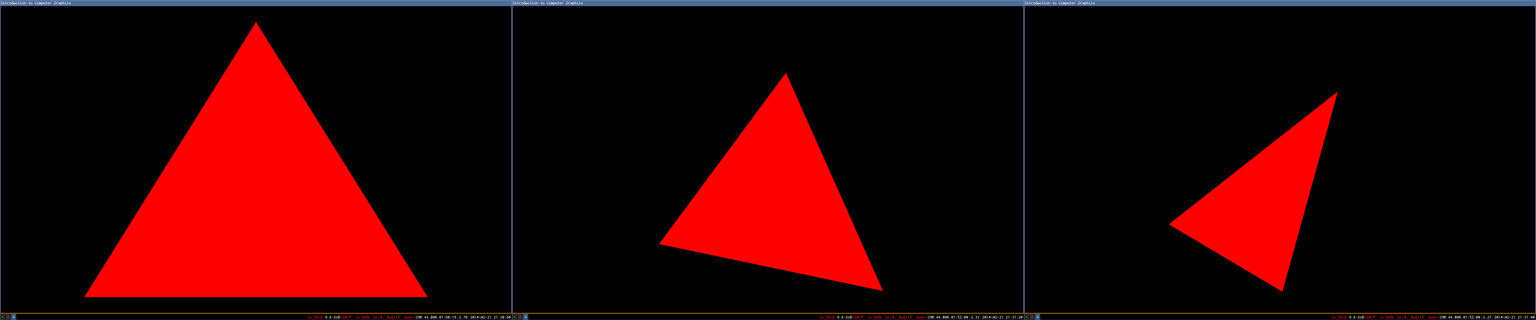
\includegraphics[scale=0.27]{figures/test.jpg}
    \caption{Screenshots of the implemention}
\end{figure}

\end{document}

